% !TeX root = ../main.tex
% Add the above to each chapter to make compiling the PDF easier in some editors.

\chapter{Related work}\label{chapter:relatedwork}

\section{Background}
In this chapter we talk about optimization, in particular the field
of linear programming, we focus on 
the  most widely used algorithms to tackle this problem,
and we present some use cases and benchmarks for this technique.

In the pipeline of query execution, cardinality estimation serves 
as a cornerstone for the optimization process. 
Cardinality, defined as the number of tuples in the output, 
plays a pivotal role in the selection of an optimal query plan. 
Modern Database Management Systems (DBMSs) often rely on 
cost-based Query Optimizers to make this selection. 
For example, the SQL Server Query Optimizer
 \parencite{microsoft2023cardinality} employs a 
 cost-based approach, aiming to minimize the estimated 
 processing cost of executing a query.

The cost estimation is influenced by two primary factors: 
the cardinality of the query plan and the algorithmic cost 
model dictated by the operators used in the query. The 
former serves as an input parameter for the latter, creating 
a dependency between the two. Enhanced cardinality estimation 
can lead to more accurate cost models, which in turn results 
in more efficient query execution plans.

  \subsection{Linear Programming}
  Linear programming or optimization is a mathematical modeling technique in which
  a linear function (called the objective function) $f(\mathbf{x}) = \sum_{j=1}^{n} c_j x_j$
  is maximized or minimized when subject to a set of constraints 
  
  \begin{align*}
  a_{11} x_1 + a_{12} x_2 + \dots + a_{1n} x_n &\leq b_1 \\
  a_{21} x_1 + a_{22} x_2 + \dots + a_{2n} x_n &\leq b_2 \\
  &\vdots \\
  a_{m1} x_1 + a_{m2} x_2 + \dots + a_{mn} x_n &\leq b_m \\
  \end{align*}
  
  Where: \(x_j\) are called decision variables for \(j = 1, 2, \ldots, n\).
  \(c_j\), \(a_{ij}\) and \(b_i\) are constants, and they constitute the coefficient vector 
  $\mathbf{c}$, the 
  constraint matrix $\mathbf{A}$ and the right-hand-side vector $\mathbf{b}$ respectively. 
  There are \(m\) constraints.
  
  The LP problem class that we are dealing with is called the packing LP problem. Additionally
  it is a special instance where:
  \begin{itemize}
      \item \( c \), the vector of the variable coefficients in the objective function,
      is a vector of all ones
      \item \( b \) , or the right hand side vector,  is a vector of all ones
  \end{itemize}
  Our specific problem is then expressed as follows:
  \begin{align}
      \text{Maximize} \quad & \sum_{j=1}^{n} x_j \notag \\
      \text{subject to} \quad & \notag \\
      & \sum_{j=1}^{n} a_{ij} x_j \leq 1, \quad & i = 1, \ldots, m \notag \\
      & x_j \geq 0, \quad & j = 1, \ldots, n \label{LP_Problem}
  \end{align}
  
  This specific class of LPs has a simple structure that we can exploit, see 
  Chapter \ref*{chapter:linearprogramming},
  to further optimize our implementation.

  \subsection{The Standard Simplex Algorithm}
  \subsubsection{The algorithm}
  
  In this subsection we will present the most widely used algorithm for solving
  LP problems. We have implemented our version  of this algorithm in the C++ language 
  and we use it, among others, to solve our dataset.
  To be approachable by the simplex algorithm, the LP \ref*{LP_Problem} needs to be cast in a 
  computational form, that fulfills the requirement of the constraint matrix having to have
  full row rank and only equality  constraints are allowed. 
  To convert the inequalities to equations, we introduce slack variables \(s_1, s_2, \dots, s_m\):

  \begin{align}
    \text{Maximize} \quad & z = \sum_{j=1}^{n} x_j \notag \\
    \text{subject to} \quad & \sum_{j=1}^{n} a_{1j} x_j + s_1 = 1 \notag \\
    & \sum_{j=1}^{n} a_{2j} x_j + s_2 = 1 \notag \\
    & \vdots \notag \\
    & \sum_{j=1}^{n} a_{mj} x_j + s_m = 1 \label{LP_Problem} \\
    & x_1, x_2, \dots, x_n, s_1, s_2, \dots, s_m \geq 0 \notag
\end{align}



  A simple packing LP in tabular form would look like this:
  \begin{equation*}
      \begin{array}{ccccccc|c}
        & a & b & c & d & s_1 & s_2 & \text{RHS} \\
        \hline
        z & -1 & -1 & -1 & -1 & 0 & 0 & 0 \\
        \hline
        s_1 & a_{11} & a_{12} & a_{13} & a_{14} & 1 & 0 & 1 \\
        s_2 & a_{21} & a_{22}& a_{23} & a_{24}& 0 & 1 & 1\\
      \end{array}
  \end{equation*}
At each iteration of the simplex method, 
we have a basic feasible solution represented by a dictionary.

\subsubsection{Example Dictionary}

\[
\begin{array}{lcl}
    x_5 & = & 10 - x_1 - 2x_2 \\
    x_6 & = & 20 - 2x_1 - 3x_2 \\
    x_7 & = & 5 - x_1 - x_3 \\
    z & = & 5x_1 + 4x_2
\end{array}
\]

In this dictionary:
\begin{itemize}
    \item \(x_5, x_6, x_7\) are basic variables.
    \item \(x_1, x_2, x_3\) are non-basic variables.
    \item The objective function value is given by the equation for \(z\).
\end{itemize}

To perform an iteration, we select an 
entering variable (e.g., \(x_1\)) and a 
leaving variable (e.g., \(x_6\)). 
We then pivot to obtain a new dictionary.

\subsection{Pivoting}

Pivoting on \(x_1\) entering and \(x_6\) leaving, 
we get a new dictionary.

  We call this a feasible dictionary\parencite{chvatal1983linear}, or a feasible tableau. This is apparent, since all
  values in the RHS are positive, and the constraint matrix $A$ also has positive coefficients.
  \begin{itemize}
      \item feasible dictionaries? 
      \item just write the algorithm in abstarct way, in the approach chapter write it in the 
      specific way I implemented it (Bland's rule, zero tolerance, ...)
      \item the grand strategy of the simplex method is that of successive improvements
      \item decision variables vs. slack variables
      \item A maximization problem is optimized when the slack variables are “squeezed out,” maximizing the true variables’ effect on the objective function. Conversely, a minimization problem is optimized when the slack variables are “stuffed,” 
      minimizing the true variables’ effect on the objective function.
      \item feasibility, boundedness, 
      \item largest coefficient rule vs. largest increase rule.
      \item the problem of stalling, degeneracy
      \item Bland's rule guarantees termination.
      
  \end{itemize}
  
  \subsubsection{The complexity}
  The Simplex algorithm for linear programming has an 
  exponential worst-case time complexity, which we denote by \( O(2^n) \).
  For packing linear programs, the worst-case time complexity of the Simplex algorithm 
  remains exponential, even though there exists polynomial time implementations for it.
  \parencite{stille2010solution}.
  

\subsubsection{Graphical interpretation}
The simplex algorithm can be understood geometrically as a 
method to navigate the vertices (corners) of a polytope 
defined by the feasible region of a linear programming problem. 
The algorithm starts at an initial vertex and moves along 
the edges of the polytope to vertices with better objective 
values until the optimal solution is reached.
\begin{center}
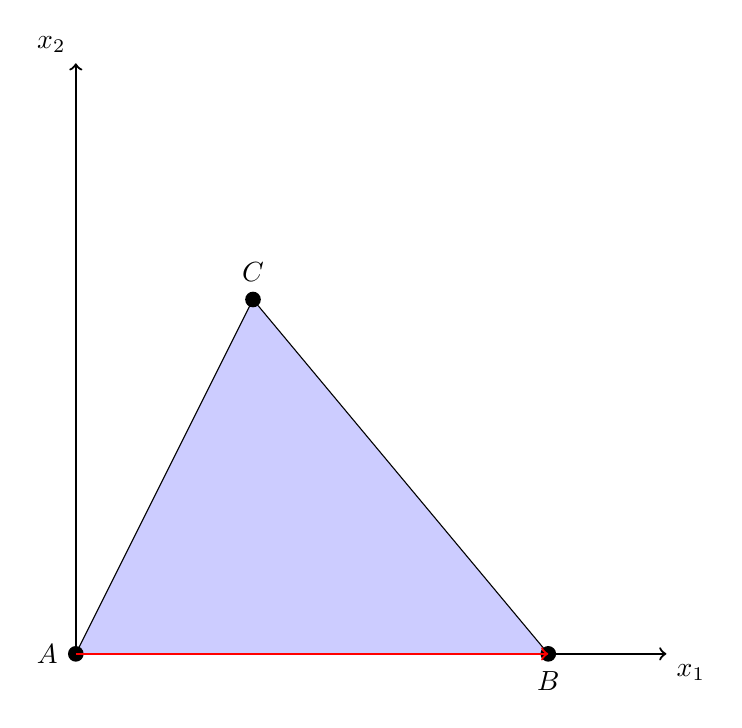
\begin{tikzpicture}[scale=1.5]
    % Draw axes
    \draw[thick,->] (0,0) -- (5,0) node[anchor=north west] {$x_1$};
    \draw[thick,->] (0,0) -- (0,5) node[anchor=south east] {$x_2$};

    % Draw polytope
    \filldraw[fill=blue!20] (0,0) -- (4,0) -- (1.5,3) -- cycle;
    
    % Label vertices
    \node at (0,0) [circle,fill,inner sep=2pt,label=left:{$A$}] {};
    \node at (4,0) [circle,fill,inner sep=2pt,label=below:{$B$}] {};
    \node at (1.5,3) [circle,fill,inner sep=2pt,label=above:{$C$}] {};

    % Draw movement of simplex algorithm
    \draw[red,thick,->] (0,0) -- (4,0);
\end{tikzpicture}
\end{center}

In the above figure, the shaded region represents 
the feasible region of a linear programming problem. 
The simplex algorithm starts at vertex \(A\) and moves to 
vertex \(B\) because \(B\) offers a better objective value. 
The algorithm would continue navigating the vertices until 
the optimal solution is found.
\begin{itemize}
    \item The simplex algorithm only evaluates the objective 
    function at the vertices of the feasible region.
    \item At each step, the algorithm selects an adjacent 
    vertex with a better objective value and moves to it.
    \item The algorithm terminates when it reaches a vertex where 
    all adjacent vertices have worse objective values, indicating an 
    optimal solution.
\end{itemize}
  \subsection{The Revised Simplex Algorithm}
  As explained in the book \parencite{chvatal1983linear}. 
  while Standard Simplex algorithm maintains and updates the entire tableau in its dense form,
   which includes both basic and non-basic variables, at each iteration. 
   In contrast, the Revised Simplex algorithm focuses on tracking only 
   the basic variables and their corresponding basis matrix $B$, 
   thereby reducing memory requirements. 
   The Revised Simplex algorithm often employs 
   the product form update method to efficiently 
   update the inverse of the basis matrix $B^{-1}$ 
   without having to recompute it from scratch, 
   making it computationally more efficient for large-scale problems. 
   Finally, we primarily use the Compressed Column Representation (CCR) of the, 
   which greatly benefits the performance of the implementation.
  \begin{algorithm}
      \caption{Revised Simplex Algorithm}
      \begin{enumerate}
          \item \textbf{Input:} A feasible basic solution, \( B \), \( c \), \( A \), and \( b \)
          \item \textbf{Output:} Optimal solution or a certificate of unboundedness
          \item Initialize \( B^{-1} \), the inverse of the basis matrix \( B \)
          \item \textbf{While True:}
          \begin{itemize}
              \setlength{\itemindent}{3em}
              \item[\textit{Step 1:}] Solve the system \( yB = c_B \) (BTRAN)
              \item[\textit{Step 2:}] Choose an entering column. This may be any column a of
              $A_N$ such that $ya$ is less than the corresponding component
              of $c_N$. If there is no such column, then the current solution is optimal.
              In other words: Choose first \( j \) such that \( c_j -yA_j > 0 \) 
              then $a=A_j$ is the enterig column.
              \item[\textit{Step 3:}] Solve the system $Bd = a$ (FTRAN)
              \item[\textit{Step 4:}] Let $x_B^{\ast} = B^{-1}b$ the current basic variables' values.
              Find the largest $t$ such that \( x_B^{\ast} - td \geq 0\)
                  if there is no such $t$, then the problem is unbounded; otherwise, at least 
                  one component of  \( x_B^{\ast} - td \) equals zero and the corresponding variable is leaving the basis.
              \item[\textit{Step 5:}] Set the value of the entering variable at 
              $t$ and replace the values $x_B^{\ast}$ of the basic variables by \( x_B^{\ast} - td \).
              Replace the leaving column of B by the entering column, and in the basis heading,
              replace the leaving variable by the entering variable.
          \end{itemize}
          
          \item \textbf{Return} Optimal solution \( B^{-1}b \)
      \end{enumerate}
  \end{algorithm} 
  
  \subsubsection*{The product form update method}
  We will discuss the PFI, introduced by George Dantzig \parencite{dantzig1954product}.
  \subsubsection*{Data structures}
  Compressed Storage Formats:
  We use the CSC format to store sparse matrices. These formats store the non-zero values, along with their corresponding row and column indices, 
  in a compact way. This reduces memory usage and speeds up operations on sparse matrices
  
  \begin{verbatim}
      struct CCRMatrix {
          float *values;  // Non-zero values in the matrix
          int *rowIdx;  // Row indices corresponding to the non-zero values
          int *colPtr;  // Points to the index in `values` where each column starts
      };
  \end{verbatim}
\subsection{Cardinality Estimation}
As previously discussed, accurate and 
reliable cardinality estimates are crucial 
in achieving faster query execution times. 
The objective is to develop a Linear Programming (LP) 
solver designed specifically for cardinality estimation. 
This solver aims to maximize a cost function that represents 
the upper bound of the output size, optimizing for both 
time and memory complexity. The performance of this solver 
will be evaluated using the Query-per-Hour Performance Metric 
(QphH@Size).

To set the stage for our implementation, 
we focus on the problem of upper-bounding the 
cardinality of a join query $Q$. 
We begin by considering the worst-case join size and then proceed
to add some constraints that keep some of our main variables in check.
 The motivation behind this work is to frame the problem of 
 estimating the size of a multi-join query as a packing 
 linear programming problem.
\subsubsection{Scenario}
To elucidate the core concepts, 
suppose we have two relation $R$ and $S$ with attributes 
\[
Q(a, b, c) = R(a, b) \Join S(b, c)
\]
where we denote the sizes of the relations as
$|R|$ and $|S|$ respectively.
It is easy to see that the largest possible output is $|R| \cdot |S|$, which occurs when the join
behaves like a cartesian product, i.e. have a selectivity equals to 1. So, this is the worst-case
upper bound.

Now the maximum sizes of these relations (i.e. the number of tuples, in our case pairs) depend on the
variables $a$, $b$ and $c$, their respective types and domains. It can also
be affected by te nature of the data or business rules.

If there are constraints on the domains of the attributes, the join size can be limited. For example:
    
\begin{itemize}
    \item If \( B \) in \( R \) and \( B \) in \( S \) have domain constraints such that they can only take on \( k \) distinct values, then the maximum number of join results for a single value of \( B \) is \( \frac{|R|}{k} \times \frac{|S|}{k} \) (assuming uniform distribution). Therefore, the worst-case join size is \( k \times \left( \frac{|R|}{k} \times \frac{|S|}{k} \right) = \frac{|R| \times |S|}{k} \).
    
    \item If there are foreign key constraints, such as \( B \) in \( S \) being a foreign key referencing \( B \) in \( R \), then each tuple in \( S \) can join with at most one tuple in \( R \). This means the worst-case join size is \( \min(|R|, |S|) \).
\end{itemize}
    
If there are multiple constraints, they can be combined to provide a tighter bound on the join size. For instance, if there's both a domain constraint and a foreign key constraint, the worst-case join size would be the minimum of the sizes derived from each constraint.

We start with the inequality \ref{eq:initial_inequality}. Applying the natural logarithm to both sides yields \ref{eq:log_inequality}. We then rename the variables, simplifying the inequality to \ref{eq:renamed_inequality}. 
Normalizing by dividing both sides by \(r'\), we obtain \ref{eq:normalized_inequality}. This leads us to the objective function for our packing LP problem.
\begin{align}
    |a| \cdot |b| &\leq |R| \label{eq:initial_inequality} \\
    \ln|a| + \ln|b| &\leq \ln|R| \label{eq:log_inequality} \\
    a' + b' &\leq r' \label{eq:renamed_inequality} \\
    \frac{1}{r'} a' + \frac{1}{r'} b' &\leq 1 \label{eq:normalized_inequality} \\
    \text{maximize } a' + b' + c' + d' \quad &\text{s.t.} \quad \frac{1}{r'} a' + \frac{1}{r'} b' \leq 1 \label{eq:objective_function}
    \end{align}

And in this simple abstracted way we get a sample packing LP from our dataset.
\subsubsection{Variables}
\subsubsection{Objective}
\subsubsection{Constraints}

\section{Previous Work}
Here we will discuss alternative approaches that are superseded by my work.
\subsection{Comparative studies of different update methods}
We will focus on one study \parencite{huangfu2015novel}.
\subsection{Other techniques}
The primal simplex method starts from a trial point that is primal feasible and iterates until dual feasibility.
The dual simplex method starts from a trial point that is dual feasible and iterates until primal feasibility.
ALGLIB implements a three-phase dual simplex method with additional degeneracy-breaking perturbation:
\begin{itemize}
    \item Forrest-Tomlin updates for faster LU refactorizations
    \item A bound flipping ratio test (also known as long dual step) for longer steps
    \item Dual steepest edge pricing for better selection of the leaving variable
    \item Shifting (dynamic perturbations applied to cost vector) for better stability
\end{itemize}
